\Chapter{Beam Line Design}%________________________________


\Section{Introduction}

Independent staging requires two beam lines, with routing of bunch trains via a kicker and septum. 
A kicker design from Indiana University (IU) was used as a base line to design a kicker specific to the
requirements at the AWA. The gap and plate length had to be determined based the beam energy, 
easily or readily available equipment, and mechanical constraints in the AWA tunnel. 
After a design was set, the kicker was fabricated. 
Two out of vacuum tests were performed to verify the fabrication process was successful.
The electronics group at the Advanced Photon Source (APS) provided equipment and help performing these tests.
The tests included a high voltage (HV) test and Time Domain Reflectometer (TDR) measurement.
Both tests were intended to verify the electrical properties of the kicker were acceptable for operation at HV.
After these tests, the kicker was installed and tested with low and high charge beams. 
A HV pulsar was borrowed from APS for the tests. 
We found the kick to be linear with respect to voltage of the pulser. 
The angle was slightly lower than simulation efforts, probably due to reflections at the
connection between the cables and kicker plates. 
The septum design was specified based on simulation work and the kicker angle.
The magnet design was completed at the Institute of Modern Physics (IMP), 
where it was also fabricated. The septum was shipped to ANL and arrived in August. 

The beamline optics also had to be determined and optimized.
The optics include four quadrupoles after the accelerating cavities, 
two quadrupoles on the bent beam line, and three focusing quadrupoles
before the PETS structure.
At first point to point matrix calculation was done to ensure that transport of the
beam was possible through the desired kicker gap.
Then an optimization was performed in using the built in GA in OPAL. 
\nrnote{assuming GA acronym will be defined in simulation chapter?}
The optimization results in several optics scenarios that can transport 
the beam through the PETS with 100\% transmission.
Next steps for the project include installation of the septum, 
down stream optics, dipole, and PETS. 
Next beam test will observe the bunch train through the kicker, 
and then through the whole beam line. 


\Section{Kicker Design Theory} \label{theory}

A fast rise time kicker is needed to separate the 
bunch trains supplied by the drive gun.  When the kicker is on, 
bunches passing though it are deflected into an alternate beam line by the kicker field.
The spacing between bunch trains is on the order of nanoseconds; 
it must be long enough to allow the kicker to reach full field before the arrival of the second bunch train, 
and also depends on the layout of the beam lines and laser timing.  
The drive beam and the accelerated `witness' beam must be synchronized so that the 
acceleration field is maximum when the witness beam arrives at the accelerating structure.
Magnetic options for transverse bunch train separation, 
such as a dipole, were disqualified due to their slow rise times 

Borrowing from a successful neighbor, a design implemented by Indiana University (IU) \cite{iukicker}
was adapted to fit the TBA requirements at the AWA. Redesign required consideration
of the length and gap between the kicker plates. Both are key parameters that determine 
what angle the beam will be deflected. Longer plates result in the beam traveling 
in the electromagnetic field for a longer time yielding a larger beam deflection angle). 
A smaller gap increases the field intensity for a given voltage (similar to a parallel plate 
capacitor), increasing the beam deflection angle. 


The kicker is essentially a parallel plate waveguide. 
A $\pm$\SI{30}{kV} power supply can be used to induce a maximum of \SI{60}{kV} potential difference 
across the plates. Each plate will be terminated in a 50 $\Omega$ load.  
The combination of the two plates will result in a static TEM mode 
between the plates. The electric field, $E_x$, and magnetic field, $B_y$,
can be derived from the voltage or current. The electric field, $E_x$, due to a potential, V, is: 
\begin{equation}
E_x=\frac{V}{h}
\end{equation}

Where h is the gap height. From Maxwell's equations, we know that the electric and magnetic 
field are related by the speed of light, c, in the case of plane and TEM waves \cite{pozar}. 
From this we can find the magnetic field induced between the plates: 
\begin{equation}
B_y=\frac{E_x}{c}
\end{equation}\label{Bv}
The electrons are traveling at nearly the speed of light, $c$, and move through the kicker on a 
trajectory perpendicular to the fields.  Plugging Equation \ref{Bv} into the Lorentz force equation, 
it is shown that the force exerted on a charge, q, 
from the electric and magnetic fields of the TEM mode are equal. 
\begin{equation}
F=q\,(E_x+v\times B_y)
\end{equation}
\begin{equation}
	F = q \,\left(E_x+c\times \frac{E_x}{c}\right)
\end{equation}

Since the force due to the electric field is equal and oriented in the same direction as the field due to the magnetic field, 
the total kick is twice that from either field alone.  
The angle induced by electric and magnetic fields has been calculated in \cite{iukicker, Wiedemann}
and is rewritten in the following terms:  
\begin{equation}
\theta_E= \frac{V\,L}{h\,T}
\end{equation}
\begin{equation}
\theta_B= \frac{B\,L}{B\rho}
\end{equation}
Where L is the plate length, and T is the kinetic energy of the beam. 
Rigidity, or $B\rho$, is a common accelerator physics term that can be found in text such as Wiedemann \cite{Wiedemann}. 
It is a convenient way to relate the magnetic field and trajectory of an energetic beam traveling through that field.
\begin{equation}
	B\rho=3.33564\,\,T\, \text{[GeV-Tesla]}
\end{equation} 
For a constant magnetic field, as the beam energy increases, the angle decreases. 
The beam is considered "rigid" at higher energies, 
and requires stronger magnetic fields to achieve the same angle, or bending radius ($\rho$).

Using the definitions above, the total angle provided by the kicker is then: 
\begin{equation}
\theta_{total}= \theta_E+\theta_B=2\theta_E=2\theta_B
\end{equation}
We can also calculate the expected deflection, or x offset after the kicker 
using geometry and the expected angle of deflection. 

\begin{equation}
	\triangle x = \left(1-\cos\left(\theta_{total}\right)\right)\rho
\end{equation}
Again, $\rho$, is the bending radius. 
\nrnote{I will add figure here showing $\rho$ and $\theta$ relationship}
\lsnote{more info needed on above equation.  What is $\rho$?  Why $1-\cos{\theta}$?}
\nrnote{$\rho$ is defined after eq 1.7, but I can repeat that.}
From these equations, we relate the design parameters gap height, length of the plates, and 
the kinetic energy of the beam. Next, further beam line considerations were included 
to narrow down what angle the kicker needed to supply. 
The largest drive beam energy achievable at the AWA is 65 MeV. 
Therefore the kinetic energy of the beam, T, was set as a constant.
Next mechanical constraints were considered. The two drive beam lines need to be separated
by at least \SI{0.5}{m} so that magnets (quadrupoles and dipoles) can fit on each 
beam line without competing for transverse space. 
\begin{figure*}
		\begin{center}		
		\begin{tikzpicture}[scale=0.7]
		\node (fig1) at (0,0)
		{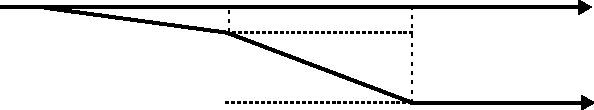
\includegraphics[width=1\textwidth]{./images/tba_geometry}};
		\node[fill=white, inner sep=2pt] (txt2) at (-5,1.3) {$\theta_k$};
		\node[fill=white, inner sep=2pt] (txt2) at (0.2,0.3) {$\theta_s$};
		\node[fill=white, inner sep=2pt] (txt2) at (5,2.5) {Beam Direction};
		\node[fill=white, inner sep=2pt] (txt2) at (5.2,0) {0.5 m};
		\node[fill=white, inner sep=2pt] (txt2) at (2,-1.5) {$\theta_d$};
		\end{tikzpicture}
		\end{center} 
	\caption{Simplified drawing of the TBA layout. 
			The angle provided by the kicker, $\theta_k$, plus the angle provided by the septum, $\theta_s$,
		    must be less than or equal to $20^\circ$.
			The two beam lines must also be at least \SI{0.5}{m} apart.}\label{fig:triangle}
\end{figure*}

Using geometry as shown in Figure \ref{fig:triangle}, an upper limit on the 
combined kicker and septum angle ($\theta_k+\theta_s$) is based on the existing dipoles at the AWA.
The maximum dipole bend angle, $\theta_d$, is $20^\circ$. 
Therefore, $\theta_{total}$  must be less than $20^\circ$. 
That way the bent beam line can be straightened out using a standard dipole, 
which is readily available at the AWA. 
It is also safer to design away from the limit of the equipment. 
Therefore a bend angle less than $20^\circ$ is preferred and allows room for tolerance errors. 
This has the added benefit of reducing energy spread. 
If the beam is bent at a smaller angle, less coherent synchrotron radiation (CSR) and energy spread will be induced.

Using the equations from Section \ref{theory}, 
a tables of possible gap, angle, and x offset values were made for comparison. 
The max beam energy was used, \SI{75}{MeV}, the expected pulsar voltage was used, \SI{35}{kV}.
A kicker lengths of \SI{0.42}{m}, \SI{0.5}{m}, and \SI{0.6}{m} were investigated.
From these calculations, the range of possible kicker angles fell between \SI{1}{^\circ} and \SI{3}{^\circ}.
The longest kicker plate option was investigated further with the understanding that 
a larger kicker angle would shorten the drift distance between the kicker and septum, 
and the results for this configuration are shown in Table \ref{kickparam}.
A shorter drift would mean less divergence in the beam before it reaches the next focusing optic (quadrupole).
\nrnote{I will reformat table later}
\begin{table}%[hbt]
	%   \vspace*{-.5\baselineskip}
	\centering
	\caption{Possible kicker parameters for a \SI{75}{MeV} beam,  
		a pulsar voltage of $\pm$ \SI{35}{kV}, 
		and kicker plate length of \SI{0.6}{m}.}
	\begin{tabular}{ccc}
		%\toprule
		\textbf{Plate Gap [mm]} & \textbf{Angle [deg]}  & \textbf{X Offset [mm]} \\
		%\midrule
		20 & 3.2   & 16.7    \\ %[3pt]
		25 & 2.57  & 13.4  \\ %[3pt]
		30 & 2.14  & 11.1 \\		 
		35 & 1.83  & 9.6	  \\
		40 & 1.6   & 8.4		 \\
		45 & 1.43  & 7.4      \\
		50 & 1.28  & 6.7   \\ %[3pt]
		%\bottomrule
	\end{tabular}
	\label{kickparam}
	%   \vspace*{-\baselineskip}
\end{table}

Next simulations were done to give an estimation of the beam size at the entrance and exit of the kicker.
Typical operating conditions at the AWA were used: accelerating cavities on crest, buck focusing at \SI{500}{A}, 
matching solenoid at \SI{255}{A}, and quadrupoles nearly in a 1:2:1 configuration with \SI{1.7}{A} and \SI{-3.3}{A}.
These are not optimized running conditions, which gives a good upper bound for how the beam will behave before tuning.
An angle of \SI{2}{^\circ} was chosen, as a reasonable starting point based on the values in Table \ref{kickparam}. 
\begin{figure}
	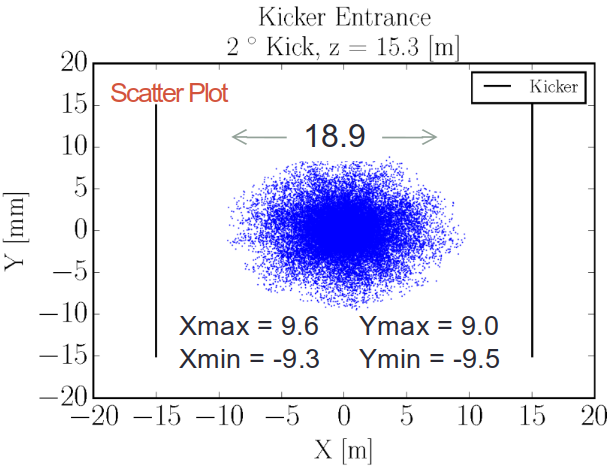
\includegraphics[width=0.5\textwidth]{./images/scatter_kicker_entrance}%
	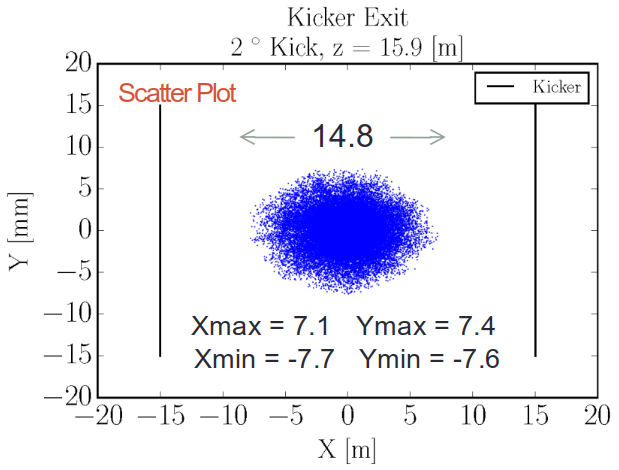
\includegraphics[width=0.5\textwidth]{./images/scatter_kicker_exit}
	\caption{Beam size of a \SI{40}{nC} beam at the entrance and exit of proposed kicker.}
\end{figure}  \label{fig:beamsizekicker}
The resulting beam sizes were about \SI{15}{mm} to \SI{19}{mm} as shown in Figure \ref{fig:beamsizekicker}. 
This requires that the kicker gap is larger than \SI{20}{mm}, 
plus room for the beam centroid deflection that the kicker will cause.
The gap needed to be large enough to allow the full width of the beam to pass through while allowing extra room
for the transverse offset of the beam as it exits the kicker. 

At this point, it was clear the gap needed to be larger than \SI{30}{mm}. 
Around this time, it was also learned that the max pulsar was $\pm$ \SI{30}{kV}, not $\pm$ \SI{35}{kV} as previously thought.
These two factors would drive the possible kick angle below \SI{2}{^\circ}, if the kicker plates remained the same length.
The next question was whether we should push for a larger angle by elongating the kicker plates, 
or if the current values at \SI{40}{mm} and above were sufficient.
A few mechanical constraints were now considered. 
Since, bent beam must travel in the same pipe as the straight through until reaching the septum, 
this requires \SI{100}{mm} (\SI{4}{inch}) beam pipe after the kicker and before the septum.
This would be a unique and custom piece designed at AWA and ordered from MDC Vacuum Products, by Scott Doran. 
This large chamber requires more vacuum pumping than other areas, 
which could complicate installation if the chamber was too long. 
In the regard, a larger angle would help.

Next, it was decided to drop the beam pipe to \SI{25}{mm} (\SI{1}{inch}) in and near the septum, 
so that the two diverging beam lines could be closer together. 
This reduces the angle and drift needed to separate the two beam lines.

At the maximum \SI{20}{^\circ} bend angle, this would put 

With the pulsar being variable between 18 and 30 kV,
Figure \ref{fig:kickerangles} and \ref{fig:kickeroffset}
both show there are several beam energies for which the above angles and beam line is feasible.
\lsnote{Those figure captions need more info, specifically, they are simulation results and some info about simulation}

the septum that will follow the kicker.
\nrnote{This section is not finished yet need to write bridge between above and following content}
\lsnote{You need to discuss the bending angle of the septum here.  Also, why is the target angle for the kicker 2 degrees?  I am not clear on that.}


For a length of \SI{1}{m}, and gap of \SI{40}{mm}, 
several beam energy and angle scenarios were considered.
As a contingency plan, it was important to consider if the 
beam energy could be lowered to still achieve the desired 
angle and x offset required in the beam line. 
\begin{figure}%[h]
	\begin{center}
		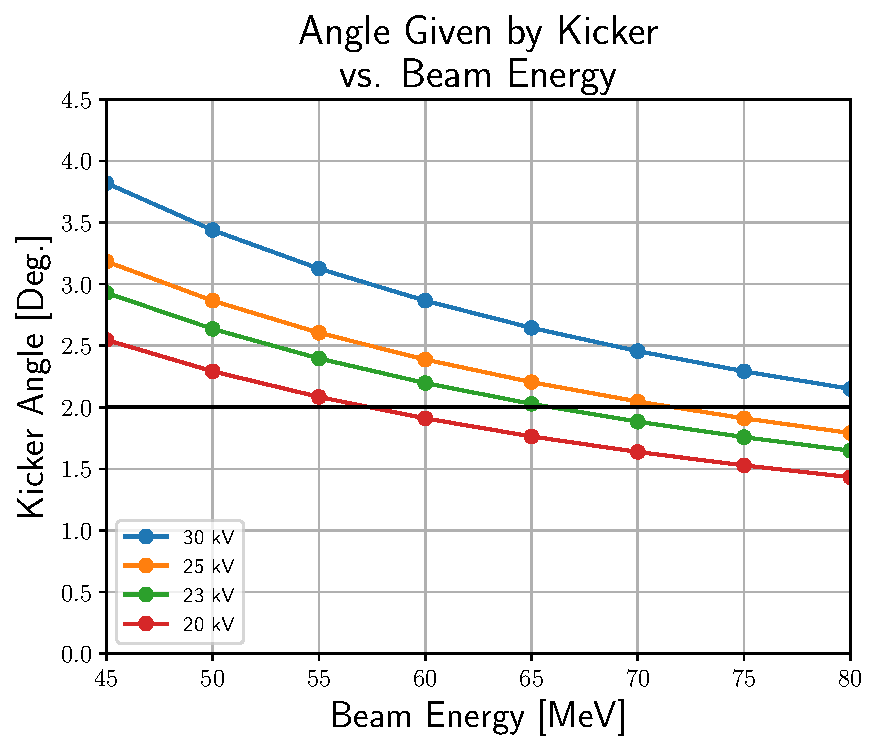
\includegraphics[width=0.65\textwidth]{./images/AngleVsEnergy}
		\caption{Calculated angle of deflection for \SI{1}{m} long 
		kicker with a gap of \SI{40}{mm} for several beam energies. The target angle is $2^\circ$.}
		\label{fig:kickerangles}
	\end{center}
\end{figure}
\begin{figure}%[h]
	\begin{center}
		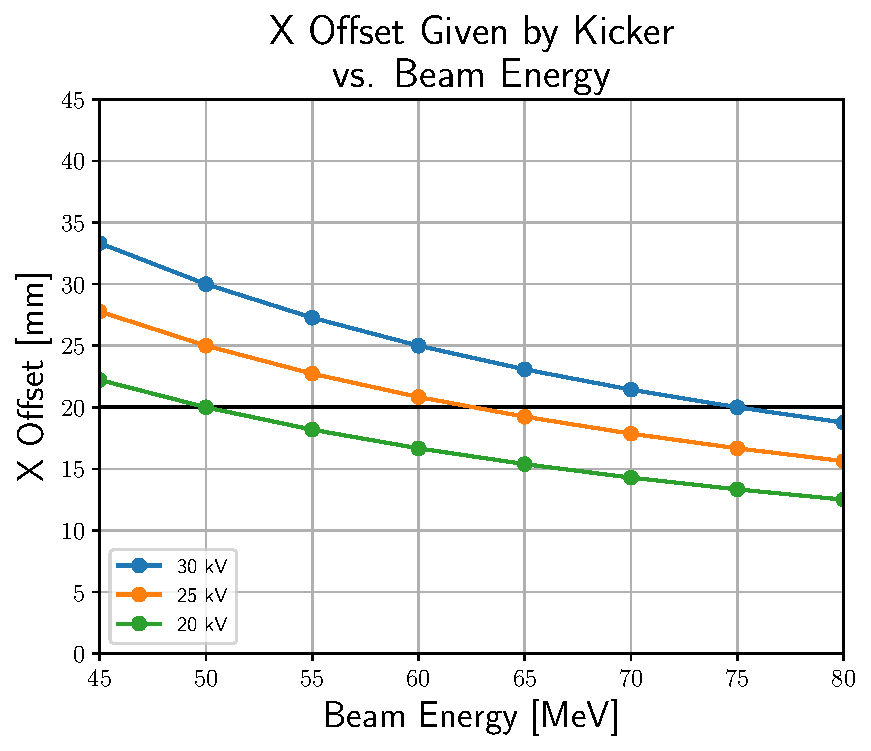
\includegraphics[width=0.65\textwidth]{./images/XoffsetVsEnergy}
		\caption{Calculated x offset of the beam after traveling
		through the \SI{1}{m} long kicker with a gap of \SI{40}{mm}.
		The target x offset is about \SI{20}{mm}.}
		\label{fig:kickeroffset}
	\end{center}
\end{figure}
\begin{figure}
	\centering
	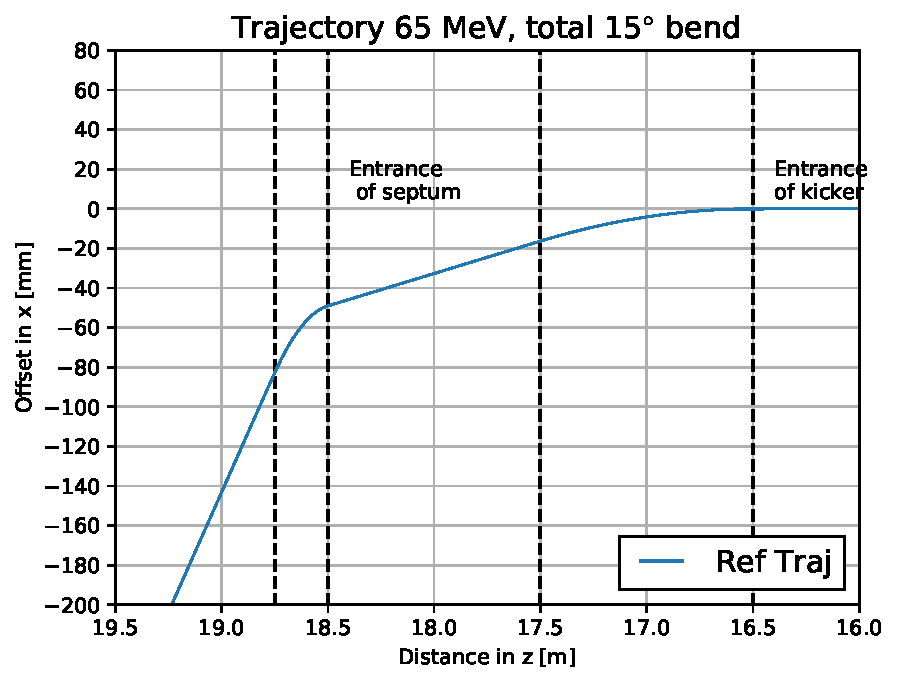
\includegraphics[width=0.65\textwidth]{./images/tba_trajectory}
	\caption{Simulation of the transverse offset of a \SI{65}{MeV} beam as 
		it travels through the proposed TBA beam line. Notice the x offset at the exit of the kicker (\SI{17.5}{m}), 
		is nearly \SI{20}{mm} as predicted in Figure \ref{fig:kickeroffset}.}
	\label{fig:beamtraj}
\end{figure}

\lsnote{I would not try to replicate the plot or the graphics.  If there are some angular deflections that you can pick off and compare to your calculation, that would be good.  But it doesn't need to be its own section.}
\nrnote{Cutting this all together because they are only impedance calculations}

\Section{Preliminary Kicker Tests}

After the design of the kicker was finalized, fabrication began at ANL.
The copper plates and ceramic brackets were fabricated on site at the ANL shops.
High voltage (HV) feedthroughs and cables were purchased from FID GmbH. 
In order to test that the fabrication of the kicker was sound, members of the 
Advanced Photon Source (APS) electronics groups graciously helped perform an 
out of vacuum AC high voltage test. Afterwards they also helped perform and 
analyze a TDR measurement of the kicker plates. \lsnote{Tell them what `TDR' stands for and what this will tell about kicker}
\begin{figure*}
	\begin{center}		
		\begin{tikzpicture}[scale=0.7]
		\node (fig1) at (0,0)
		{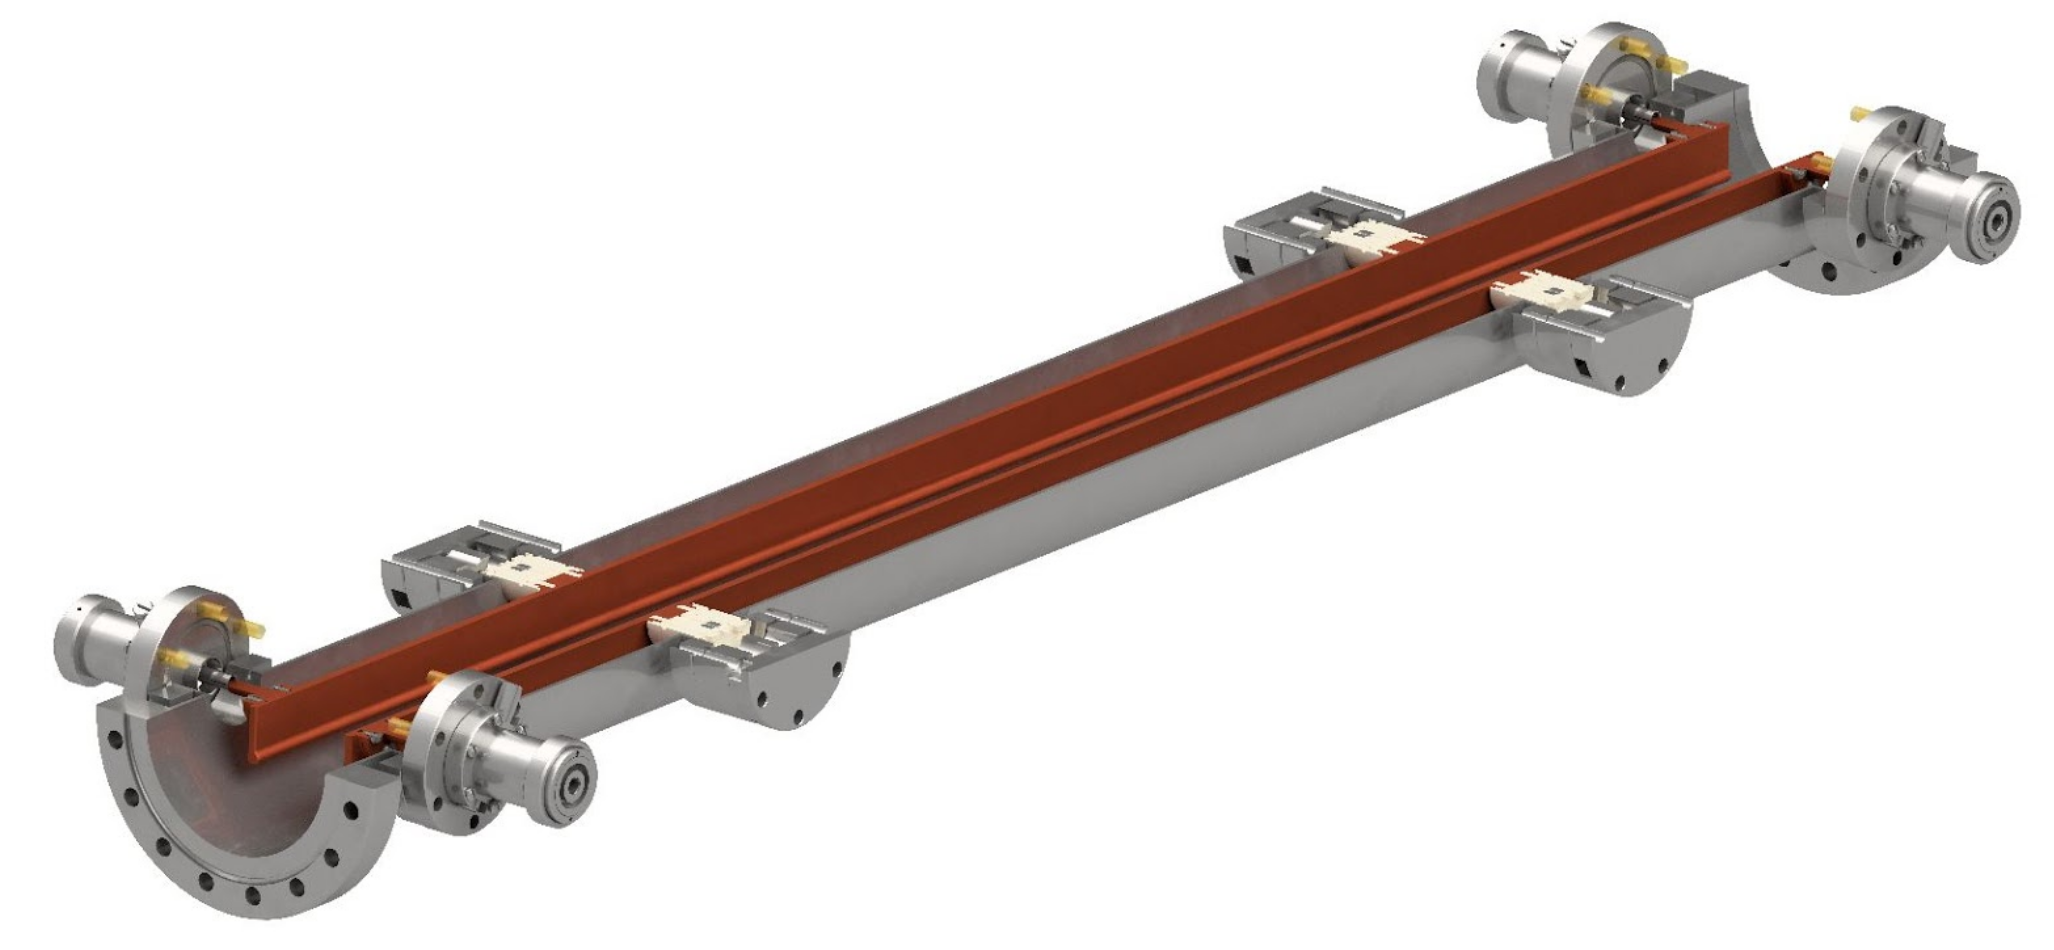
\includegraphics[width=1\textwidth]{./images/kicker}};
		\node[fill=white, inner sep=2pt] (txt2) at (-10,0) {Port 1};
		\node[fill=white, inner sep=2pt] (txt2) at (-5, -5) {Port 3};
		\node[fill=white, inner sep=2pt] (txt2) at (5.5,6) {Port 2};
		\node[fill=white, inner sep=2pt] (txt2) at (10,1) {Port 4};
		\end{tikzpicture}
	\end{center} 
	\caption{CAD drawing of AWA kicker design, courtesy of Scott Doran from AWA.
	Ports are connected the HV cables purchased from FID GmbH. 
	Power is suppled by a puslar also fabricated by FID GmbH and borrowed from the APS Electronics group.}
\end{figure*}\label{fig:AWAkicker}
\begin{figure}%[h]
	\begin{center}
		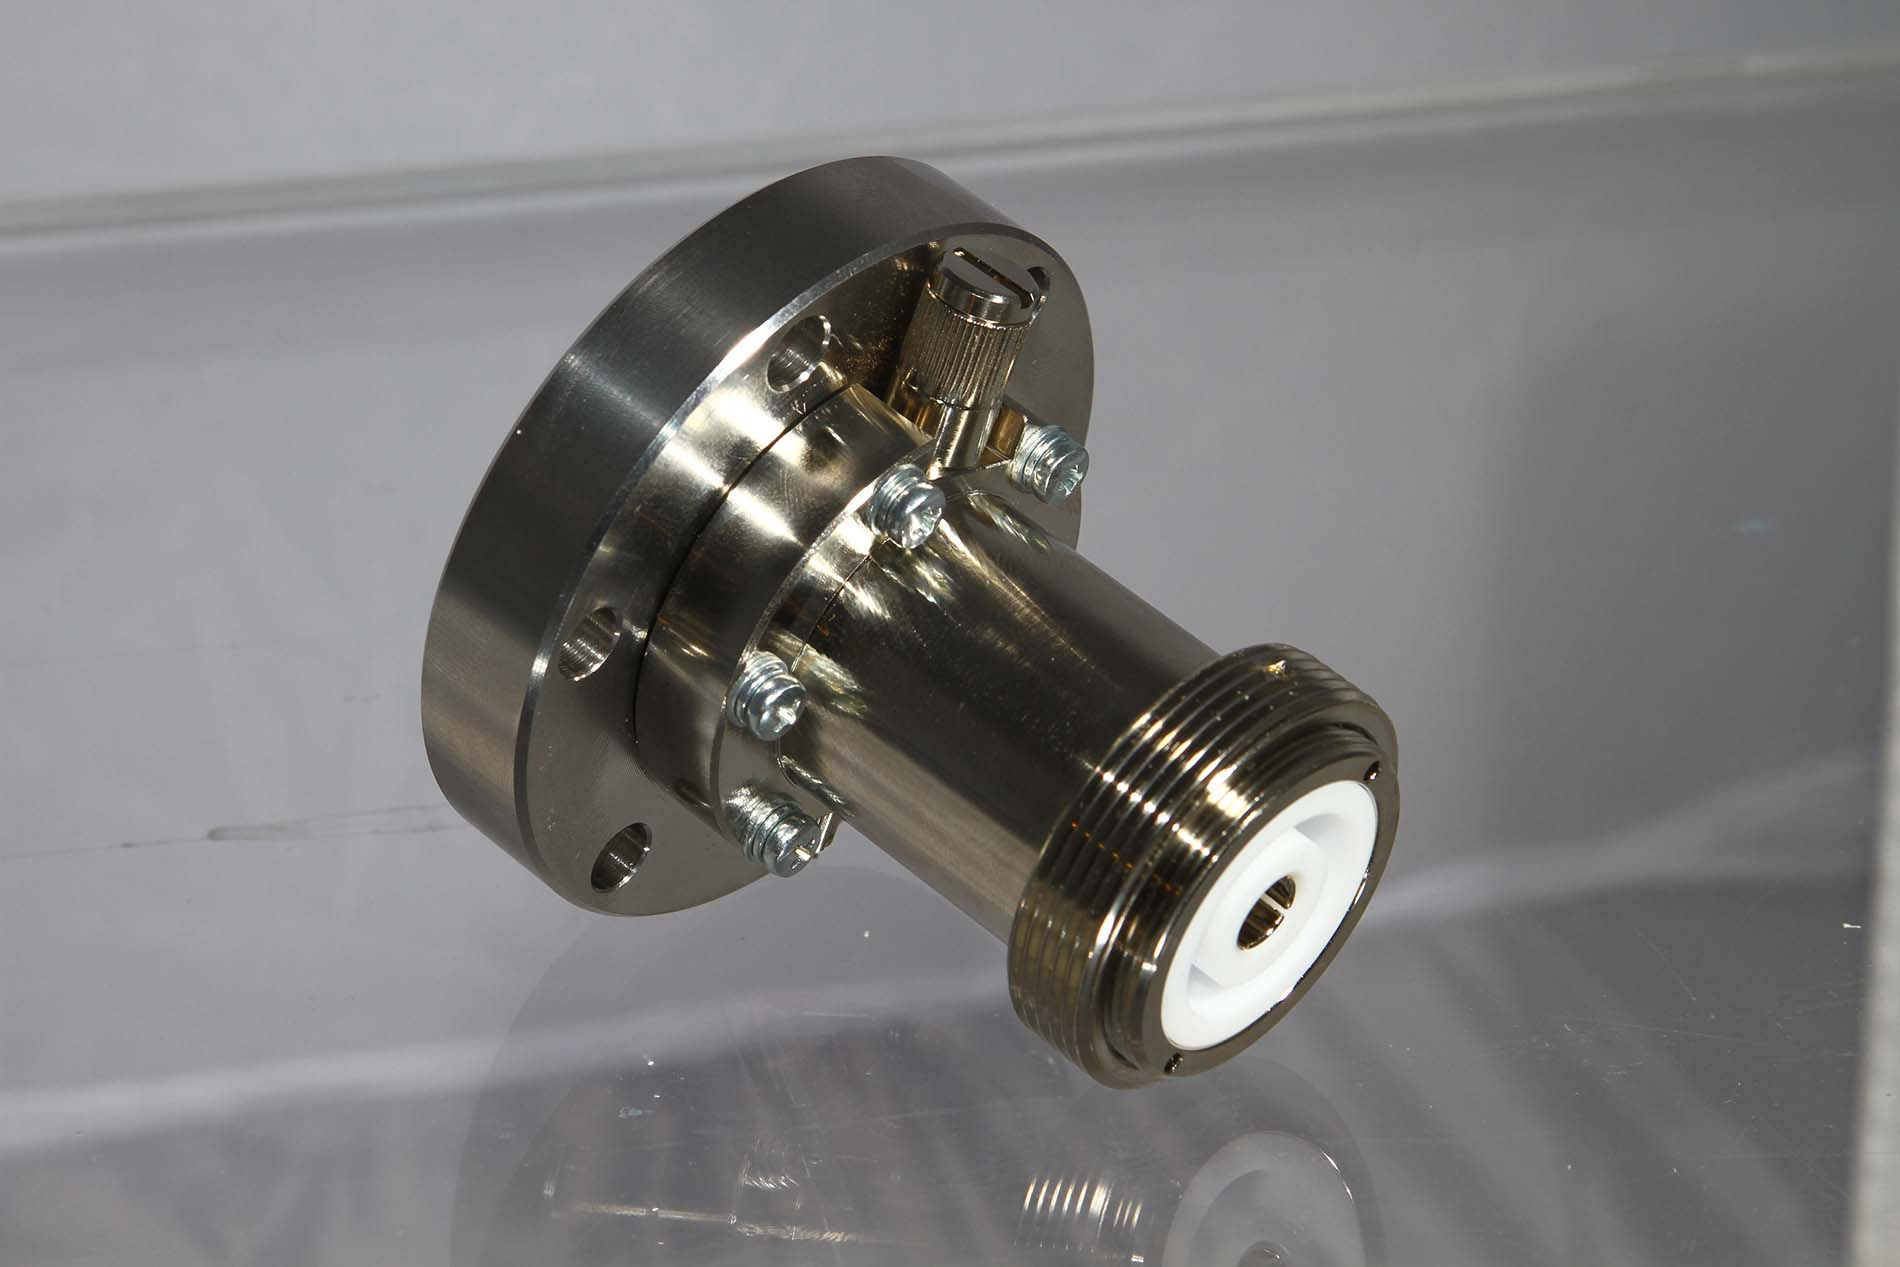
\includegraphics[width=0.5\textwidth]{./images/FID_feedthrough1}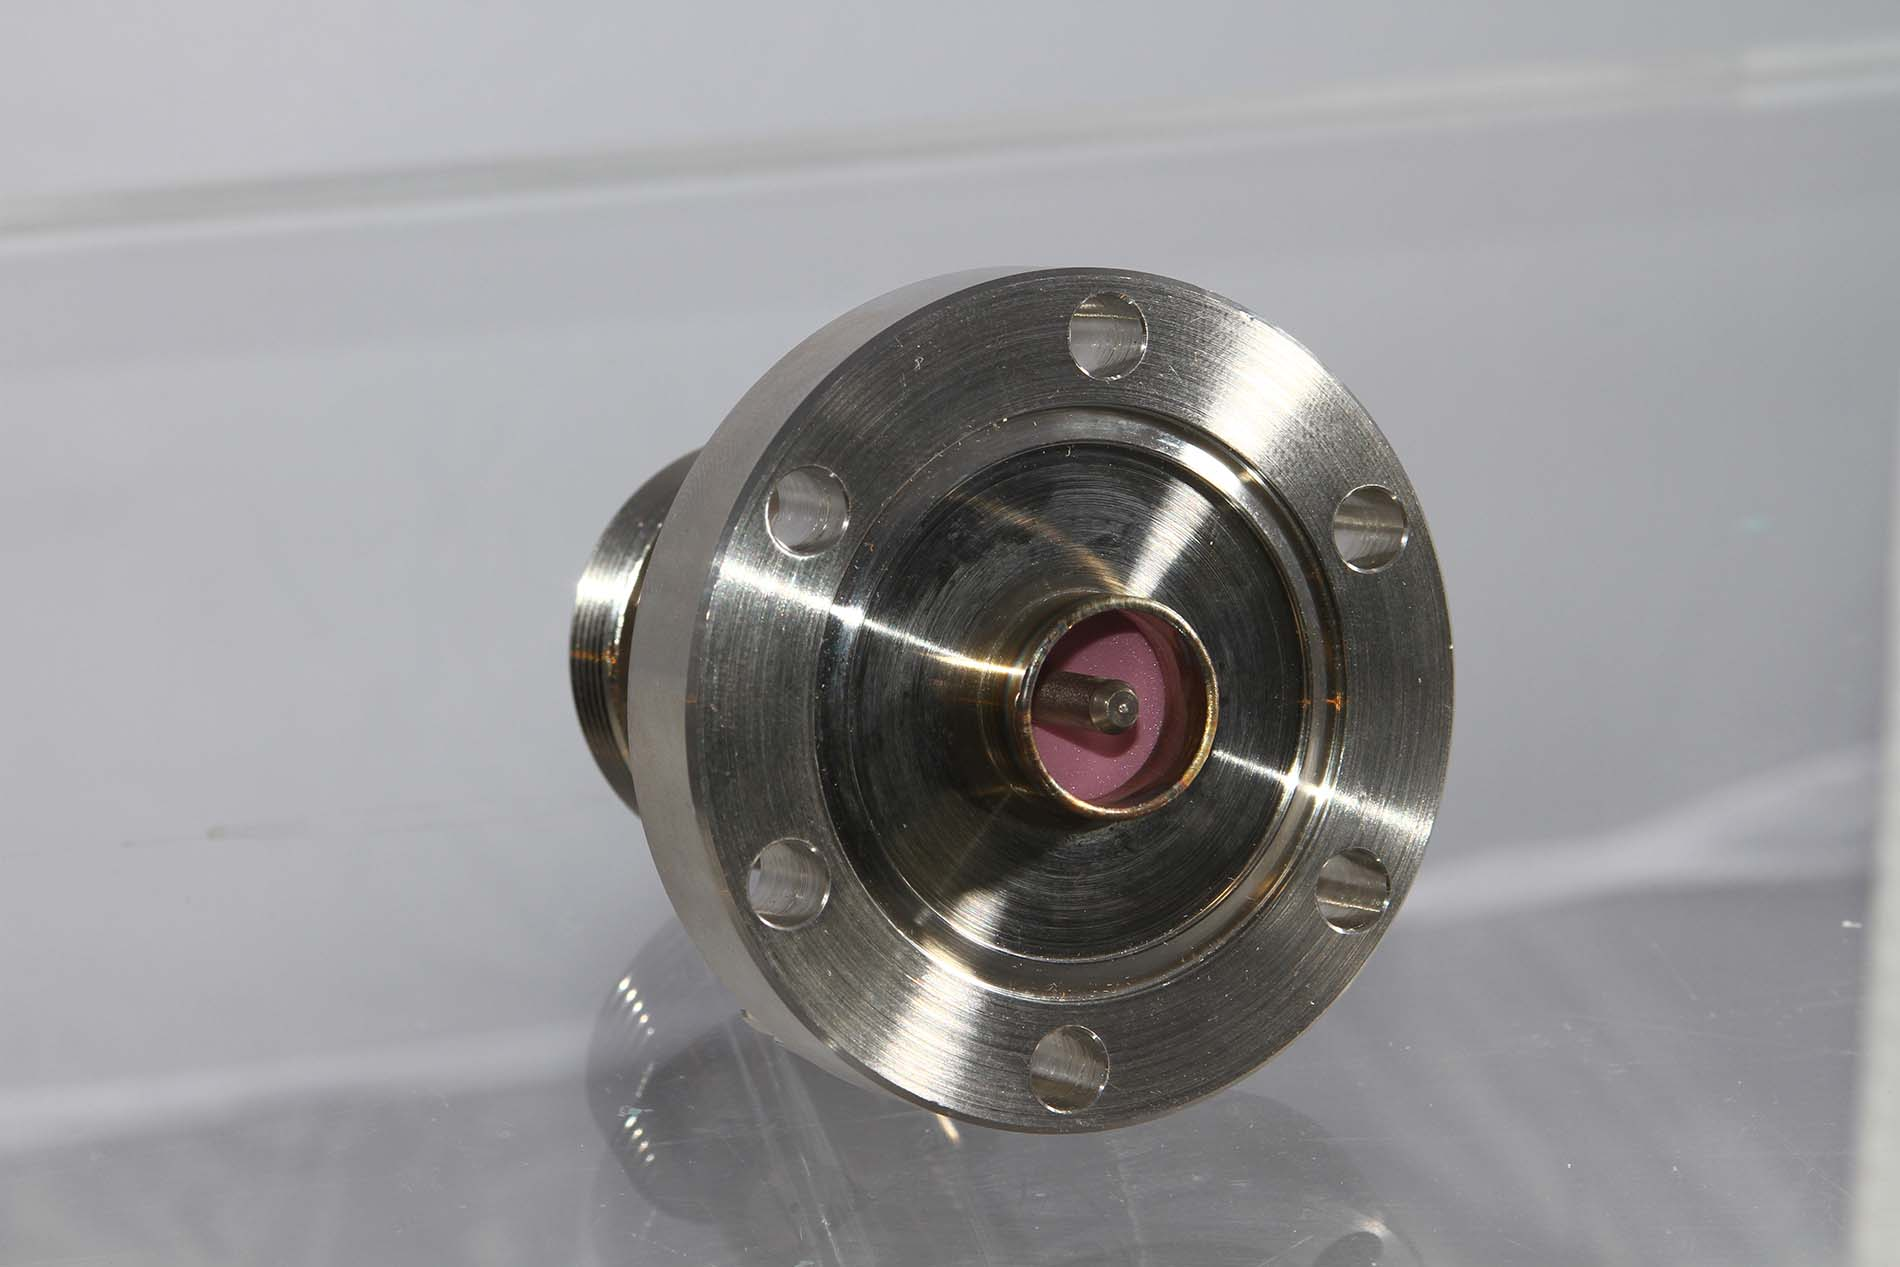
\includegraphics[width=0.5\textwidth]{./images/FID_feedthrough2}
		\caption{High voltage feedthrough purchased from FID GmbH. Left, connection to the HV cables.
		Right, the in vacuum pin that connects to the copper kicker plates.}
		\label{fig:feedthroughs}
	\end{center}
\end{figure}


\Subsection{High Voltage Kicker Test}
Two HV tests were performed at the APS. \lsnote{For what purpose?}
The first test consisted of HV applied in increments to ports 3 and 4 on the kicker.  \lsnote{Label the ports in the figure.}
Ports 1 and 2 were shorted to ground. There was no leakage current up to \SI{8}{kV} RMS.
The second test reversed the set up with 3 and 4 grounded and ports 1 and 2 exposed. 
There was no leakage current up to \SI{9}{kV} RMS, which was the maximum voltage of the test equipment.
Figure~\ref{fig:AWAHVkicker} shows the connection and location of the kicker in the APS Faraday cage.
\begin{figure}%[h]
	\begin{center}
		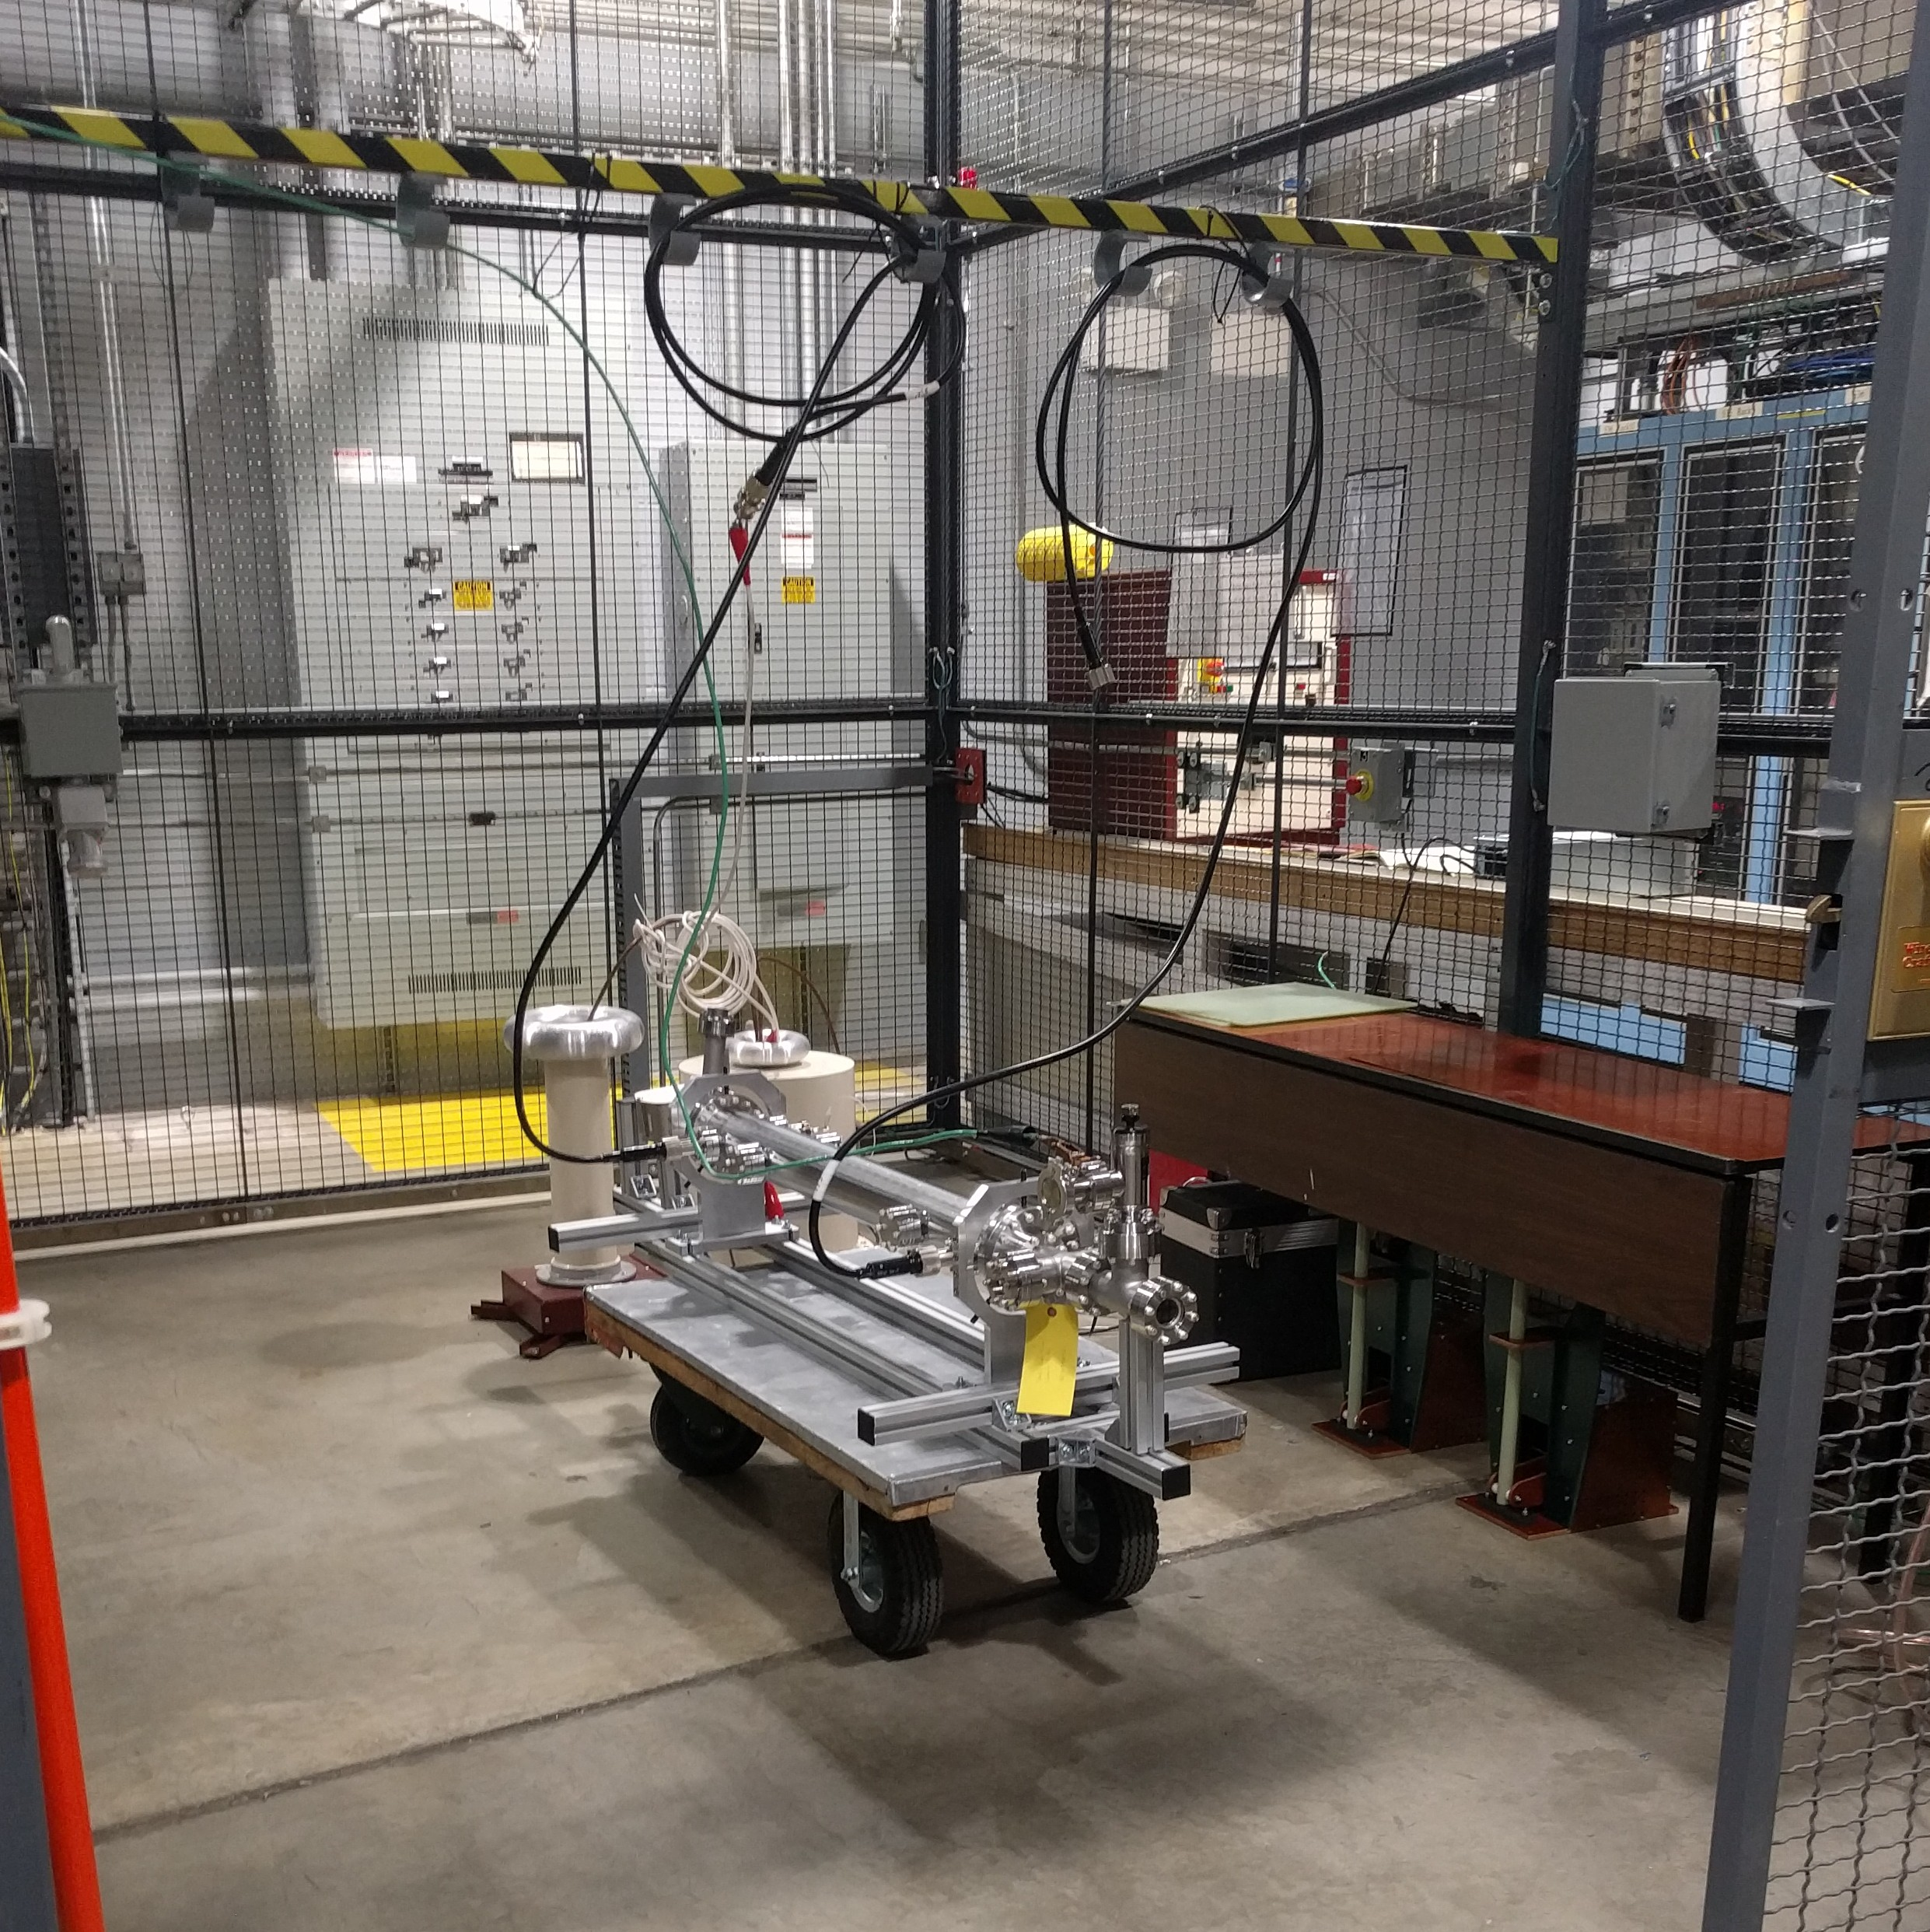
\includegraphics[width=0.65\textwidth]{./images/kicker1}
		\caption{High voltage test cage at the APS. 
			The kicker was grounded on one side and exposed to HV AC power on the other. 
			The Faraday cage was closed during testing. }
		\label{fig:AWAHVkicker}
	\end{center}
\end{figure}


\Subsection{Time Domain Reflectometer Test}
After the HV test was completed, a Time Domain Reflectometer (TDR) measurement was preformed at the APS [], 
with the help of C. Y. Yao, A. Brill, X. Sun and C. Jing.
This technique measures reflections along a conductor and gives information about discontinuties in the line being measured. 
This information was used to determine the impedance along the cables, feedthroughs, and plates of the kicker. 
Ideally, the response would be \SI{50}{\ohm} to reduce the amount of reflections and resulting power loss. 
The measurements, plotted by C.Y. Yao in Figure \ref{fig:TDR}, show a larger impedance at the feedthrough locations.
Due to resource and time constraints, it was a goal to use off the shelf parts where possible in fabrication of the kicker.
Therefore, the feedthrough mismatch is expected because they were not specifically designed to couple to the plate geometry.
A substantial amount of time and resources were spent to minimize reflections for the APS kickers plotted in Figure \ref{fig:APS-kicker}.
However, that kicker still devates from \SI{50}{\ohm} near the feedthroughs.
Given this comparison to the kickers fabricated at the APS, C. Y. Yao advised the mismatch we observed was not dangerous to 
the pulsar or cables that would drive the kicker.  
The only negative result is the reduced amount of voltage supplied to the plates, and therefore, a reduction in the kick given to the beam.
\begin{figure*}
	\centering
	\begin{subfigure}{0.75\textwidth}
		\centering
		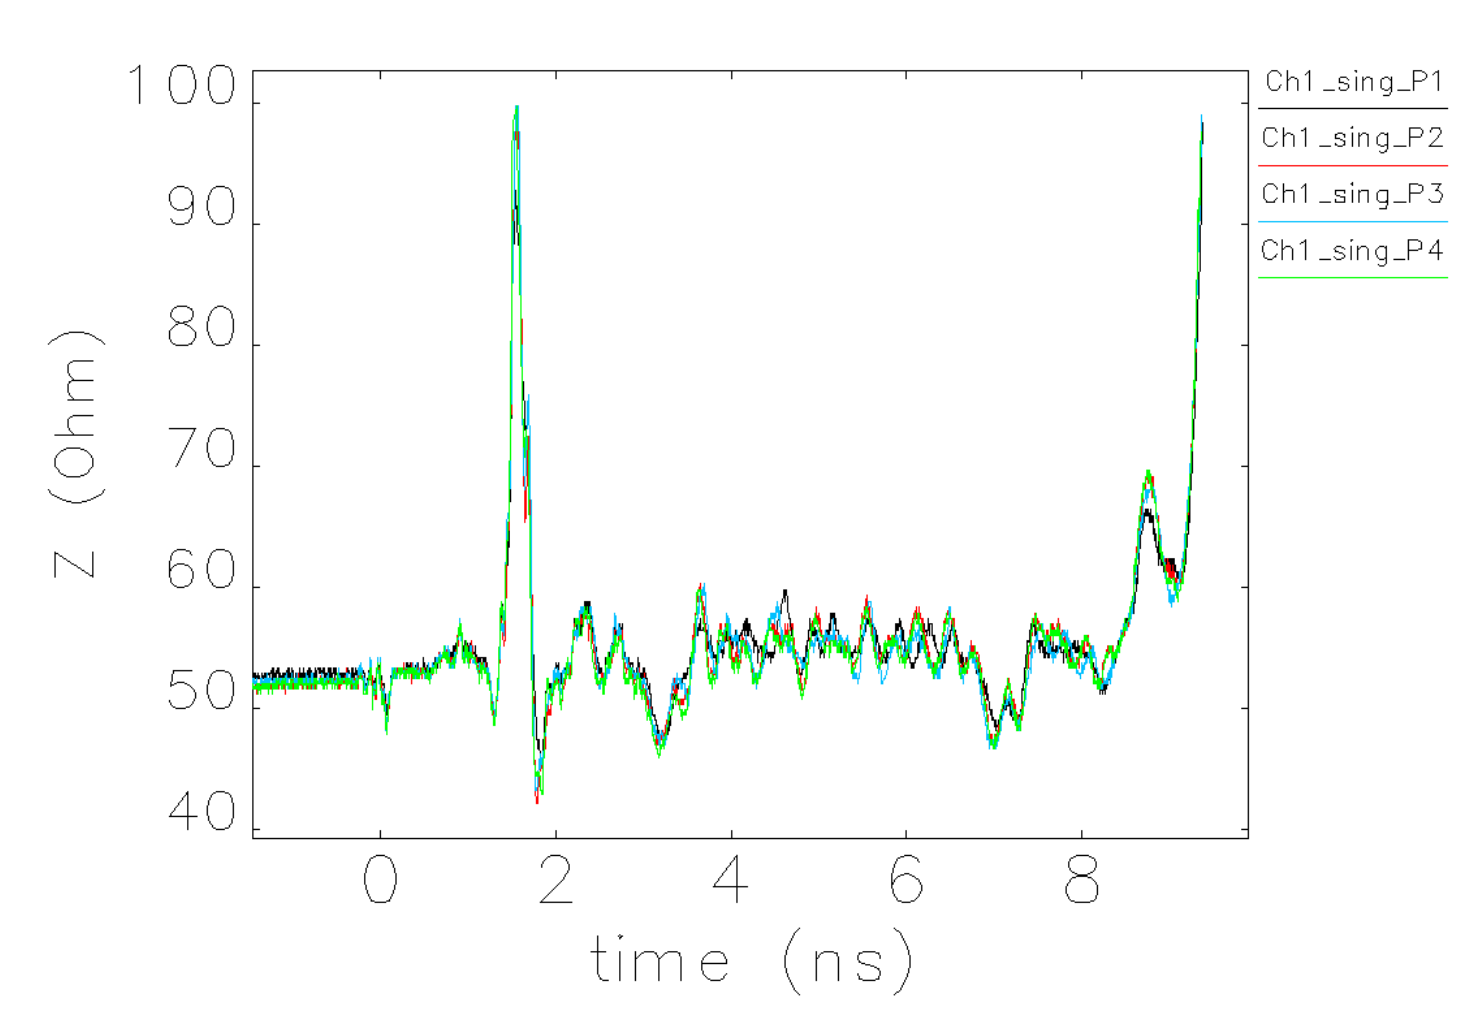
\includegraphics[width=\textwidth]{./images/TDR_AWA_kicker}
		\caption{TDR single mode measurements of AWA kicker.}
		\label{fig:AWA-kicker}
	\end{subfigure}
	~%add desired spacing between images, e. g. ~, \quad, \qquad, \hfill etc. 
	%(or a blank line to force the subfigure onto a new line)
	\begin{subfigure}{\textwidth}
		\centering
		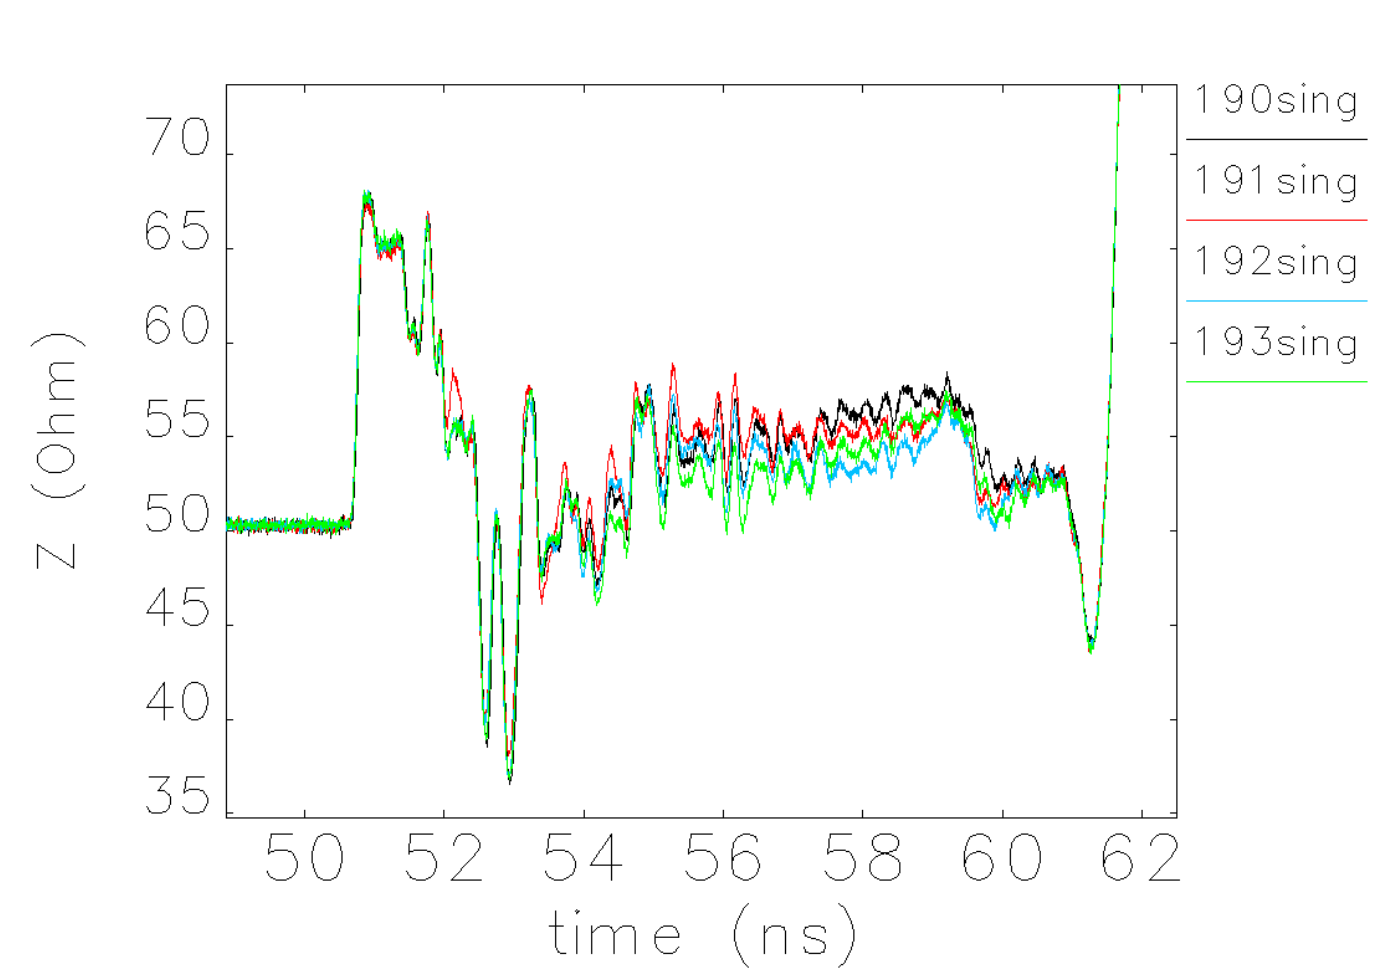
\includegraphics[width=0.75\textwidth]{./images/TDR_APS_kicker}
		\caption{TDR single mode measurements of APS kicker.}
		\label{fig:APS-kicker}
	\end{subfigure}
	\caption{TDR measurements of AWA and APS kickers, plotted by C. Y. Yao. 
	Single mode refers to the orientation of the measurement. 
	Only one port of the kicker is driven and measured at a time. 
	\nrnote{caption ok??}}\label{fig:TDR}
\end{figure*}

\Section{Measurment of Beam Deflection}

Next the kicker was installed in the AWA drive beam line.
It's approximate location is 16.5 meters downstream of the cathode.
The HV pulsar was located on the roof of the bunker.

\nrnote{todo}



\Section{TBA Beam Line}
\lsnote{Where are you going with this?  Before you spend a lot of time on it, what are your goals here?}
A drift: 
\begin{equation}
R_d = 
\begin{bmatrix}
1 & L \\
0 & 1
\end{bmatrix}
\end{equation}

A quad: 
\begin{equation}
R_q = 
\begin{bmatrix}
1 & 0 \\
\pm \frac{1}{f} & 1
\end{bmatrix}
\end{equation}

A dipole:
\begin{equation}
R_s = 
\begin{bmatrix}
a & b \\
c & d
\end{bmatrix}
\end{equation}

To convert from focal length to quadrupole strength we must take into account the 
beam energy as well as the dimensions of the quadrupole. 
\begin{equation}
	\frac{1}{f} = kl \\
\end{equation}
Where $l$ is the quadrupole's effective length, and k is the gradient w.r.t 
the beam energy and magnet strength \cite{Wiedemann}:
\begin{equation}
	k = \SI{0.2998}{} \frac{g[\SI{}{T/m}]}{p [\SI{}{GeV/c}]}\label{k}
\end{equation}



 To reduce the number of free parameters quickly without using expensive PIC simulations, 
 the transfer matrix of the beam line was considered. Starting at the end of the linac, 
 we consider the first four quadrupoles before the kicker. All the quadruple strengths (4) and
 distances between the quadrupoles (6) are parameters under consideration. To reduce the number
 of variables from 10 to 4, we use the quadruplet telescope module as described by K. Brown in \cite{brown}.  The transfer matrix R, is reduced to:  
 \begin{equation}
 R_q = R_{d4} \cdot R_{q3} \cdot R_{d3} \cdot R_{q2} \cdot R_{d2} \cdot R_{q1} \cdot R_{d1} = 
 \begin{bmatrix}
 \frac{f_2 f_4}{f_1 f_3} & 0 \\
 0 & \frac{f_1 f_3}{f_2 f_4}	
 \end{bmatrix}\label{kb1}
 \end{equation}

\nrnote{add detail about this matrix comes from and expand matrix to x and y}
Where $f_1 \ldots f_4$ stand for the focal lengths of each quad before the kicker. 
Due to other experiments in the AWA tunnel, 
the first quadrupole was required to be at least $\SI{3}{m}$ away from the exit of the 
last accelerating cavity in the linac. This gives the initial drift length and value
for $f_1$. 

\Subsection{Point to Point Check}
To achieve point to point transport of the beam, we can 
equate $f_1 = f_4$ and $f_2 = f_3$. This reduces Eq. \ref{kb1} to:
 \begin{equation}
R_q =
\begin{bmatrix}
1 & 0 \\
0 & 1	
\end{bmatrix}
\end{equation}
We can further simplify the experimental set up by 
assuming $f_1=f_2$. Given the total distance, D, available for the
quads in the beam line, \SI{3.8}{m}, we can then solve
for the focal length $f_1$: 
\begin{align}
	D = 4f_1 + 4 f_2 = 8f_1 = \SI{3.8}{m} \\
	f_1 = \SI{0.475}{m}
\end{align}
Given an energy of \SI{65}{MeV}, a quadrupole length of \SI{11}{cm}, 
and Eq. \ref{k} we can calculate this configuration would require a 
magnet strength of \SI{4.14}{[T/m]}. This is feasible considering the 
max strength is \SI{9}{[T/m]}.

To determine the effect of this configuration on the beam size and divergence
we compare the sigma matrix before and after the qudrupoles:
\begin{align}
	\sigma_1 = R\cdot \sigma_0 \cdot R^T \\
	= 
	\begin{bmatrix}
	1 & 0 \\
	0 & 1	
	\end{bmatrix}
	\begin{bmatrix}
	1 & 0 \\
	0 & 1	
	\end{bmatrix}
    \begin{bmatrix}
	1 & 0 \\
	0 & 1	
	\end{bmatrix} \\
	=
	\begin{bmatrix}
	1 & 0 \\
	0 & 1	
	\end{bmatrix}
\end{align}

\Subsection{Point to Parallel Configuration}
Having less divergence entering the kicker may be more beneficial than 
maintaining the initial beam distribution. 

\iffalse 
 \[
 \begin{bmatrix}
 x_{11}       & x_{12} & x_{13} & \dots & x_{1n} \\
 x_{21}       & x_{22} & x_{23} & \dots & x_{2n} \\
 \hdotsfor{5} \\
 x_{d1}       & x_{d2} & x_{d3} & \dots & x_{dn}
 \end{bmatrix}
 =
 \begin{bmatrix}
 x_{11} & x_{12} & x_{13} & \dots  & x_{1n} \\
 x_{21} & x_{22} & x_{23} & \dots  & x_{2n} \\
 \vdots & \vdots & \vdots & \ddots & \vdots \\
 x_{d1} & x_{d2} & x_{d3} & \dots  & x_{dn}
 \end{bmatrix}
 \]
 \fi
 
 \Section{TBA Beam Line Optimization Results}